\documentclass[12pt]{article}
\usepackage[a4paper, bindingoffset=0.2in, %
							left=0.5in,right=0.5in,top=0.5in,bottom=0.5in,%
							footskip=.25in]{geometry}
\usepackage{graphicx}
\usepackage{listings}
\usepackage{amssymb}
\usepackage{amsmath}
\usepackage{hyperref}


\title{PSet5 Report}
\author{Ali Abolhassanzadeh Mahani}

\begin{document}
	\maketitle
	\section{Generating Uniform Random Numbers}
	As we expected the amount of numbers generated for each digit is about $\frac{N}{10}$. Fig\ref{fig:p1_hist}
	\begin{figure}[h!]
		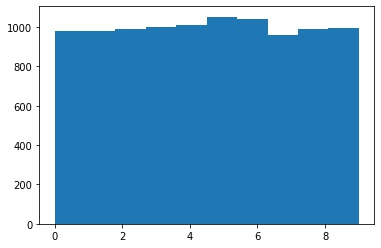
\includegraphics[width=0.9\linewidth]{../p1_hist.jpg}
		\label{fig:p1_hist}
		\caption{Hist plot of N numbers generated uniformly from 0 to 9}
	\end{figure}
	I plotted the equation and as expected we see that the equation holds for this generator.
	
	This is very similar to the Random walk --random generation-- in which both express the cenetral limit property. Fig\ref{fig:p1_plot}
	\begin{figure}[h!]
	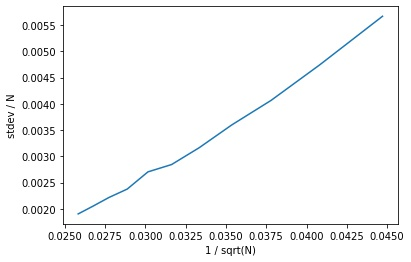
\includegraphics[width=0.9\linewidth]{../p1_plot.jpg}
	\label{fig:p1_plot}
	\caption{plot to show the expression of central limit phenomena}
\end{figure}

	\section{Entanglement}
	Did what the question asked me to do and got the uniform distribution histogram again, meaning that
	there are no entanglements. Fig\ref{fig:p2}
	\begin{figure}[h!]
		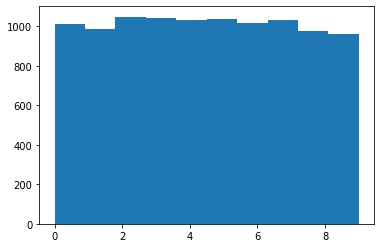
\includegraphics[width=.9\linewidth]{../p2.jpg}
		\label{fig:p2}
		\caption{The uniform plot after plotting the histogram for numbers generated after every 4}
	\end{figure}
	
	\section{Central Limit Theorem}
	I generated rands with the length of N and summed them to get to the central limit theorem.
	The hist plots are available in Fig\ref{fig:p3}
	\begin{figure}[h!]
		\centering
		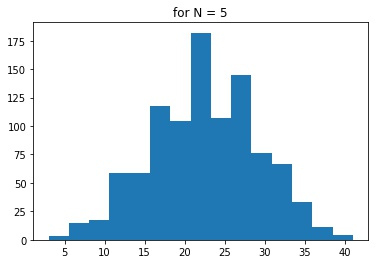
\includegraphics[width=.4\linewidth]{../p3_5.jpg}
		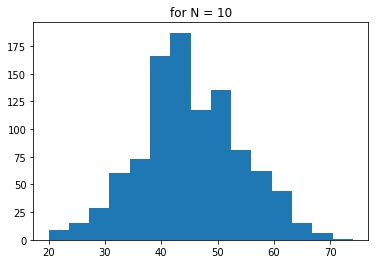
\includegraphics[width=.4\linewidth]{../p3_10.jpg}
		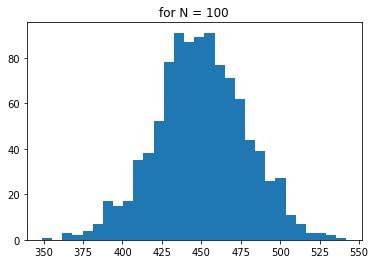
\includegraphics[width=.4\linewidth]{../p3_100.jpg}
		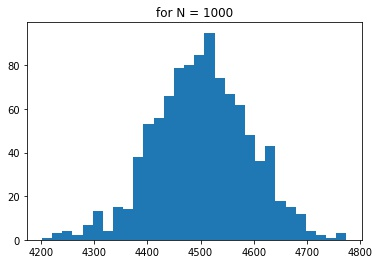
\includegraphics[width=.4\linewidth]{../p3_1000.jpg}
		\label{fig:p3}
		\caption{Central limit for lengths of 5, 10, 100, 1000}
	\end{figure}
	In all these exercises we witness that the higher the size N, the nearer the distribution is to a gaussian function.

	\section{Transforming the Distribution Function}
	I used the method seen in the code to generate the gaussian distribution in 2 dimentions.
	Here are the results for different numbers. Fig\ref{fig:p4}
	\begin{figure}[h!]
		\centering
		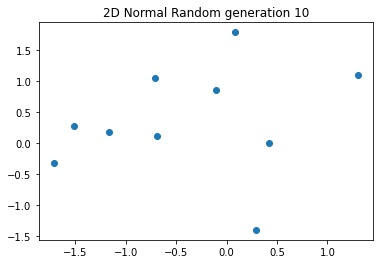
\includegraphics[width=.45\linewidth]{../p4_10}
		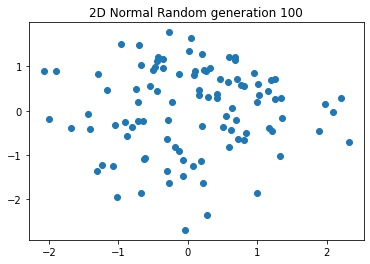
\includegraphics[width=.45\linewidth]{../p4_100}
		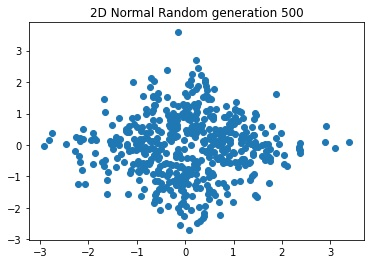
\includegraphics[width=.45\linewidth]{../p4_500}
		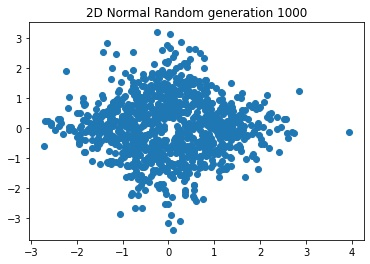
\includegraphics[width=.45\linewidth]{../p4_1000}
		\label{fig:p4}
		\caption{2 dimentional normal distribution for sizes 10, 100, 500, 1000}
	\end{figure}


	
	
	
	
	
\end{document}